\documentclass[11pt,a4paper]{article}

% --- Packages ---
\usepackage[utf8]{inputenc}
\usepackage[margin=1in]{geometry}
\usepackage{amsmath,amssymb,amsfonts}
\usepackage{booktabs}
\usepackage{tabularx}
\usepackage{xcolor}
\usepackage{graphicx}
\usepackage{hyperref}
\usepackage{listings}
\usepackage{fancyhdr}
\usepackage{enumitem}
\usepackage{tcolorbox}
\usepackage{caption}
\usepackage{microtype}

% --- Graphics Path ---
\graphicspath{{images/}}

% --- Hyperref Setup ---
\hypersetup{
    colorlinks=true,
    linkcolor=blue!70!black,
    citecolor=blue!70!black,
    urlcolor=blue!70!black,
    pdftitle={QuietSpace: Comprehensive System Architecture & Engineering Report},
    pdfauthor={Senior Design Team, North Carolina A&T State University}
}

% --- Code Listings Setup ---
\definecolor{codegreen}{rgb}{0,0.6,0}
\definecolor{codegray}{rgb}{0.5,0.5,0.5}
\definecolor{codepurple}{rgb}{0.58,0,0.82}
\definecolor{backcolour}{rgb}{0.96,0.97,0.98}
\definecolor{deepnavy}{rgb}{0.06,0.15,0.35}

\lstdefinestyle{quietcode}{
    backgroundcolor=\color{backcolour},
    commentstyle=\color{codegreen},
    keywordstyle=\color{deepnavy}\bfseries,
    numberstyle=\tiny\color{codegray},
    stringstyle=\color{codepurple},
    basicstyle=\ttfamily\footnotesize,
    breakatwhitespace=false,
    breaklines=true,
    captionpos=b,
    keepspaces=true,
    numbers=left,
    numbersep=7pt,
    showspaces=false,
    showstringspaces=false,
    showtabs=false,
    tabsize=2,
    frame=single,
    rulecolor=\color{black!15}
}
\lstset{style=quietcode}

% --- Header and Footer ---
\pagestyle{fancy}
\fancyhf{}
\rhead{\footnotesize QuietSpace System Report --- NCAT Senior Project}
\lhead{\footnotesize F.D. Bluford Library Monitoring}
\cfoot{\thepage}

% --- Custom Colored Boxes ---
\newtcolorbox{calloutbox}[1]{
    colback=blue!5!white,
    colframe=deepnavy,
    fonttitle=\bfseries,
    title=#1,
    arc=3mm
}

\newtcolorbox{alertbox}[1]{
    colback=red!5!white,
    colframe=red!70!black,
    fonttitle=\bfseries,
    title=#1,
    arc=3mm
}

% --- Document Information ---
\title{
    \vspace{-1.0cm}
    \begin{center}
        
\includegraphics[width=0.48\textwidth]{images/logo.png} \\[0.3cm]
    \end{center}
    \textbf{\Huge QuietSpace} \\[0.3cm]
    \Large Real-Time Study Room Noise Monitoring \& Incident Escalation System \\[0.2cm]
    \large \textbf{Comprehensive System Architecture, Technical Specification, and Engineering Roadmap}
}

\author{
    \textbf{Senior Design Project Team} \\[0.1cm]
    Department of Computer Science \\
    North Carolina A\&T State University (NCAT) \\[0.1cm]
    \textit{Deployment Target: F.D. Bluford Library (3rd Floor Study Rooms 311, 312, 313)}
}

\date{Academic Year 2025--2026 $\cdot$ October 2026}

\begin{document}

\maketitle

\begin{abstract}
\noindent \textbf{QuietSpace} is an autonomous, event-driven IoT and web platform engineered to resolve acoustic disruptions in university library study environments. Developed as a Senior Design Capstone at North Carolina A\&T State University (NCAT), the platform addresses the persistent challenge of noise enforcement in group study rooms (specifically Rooms 311--313 of the F.D. Bluford Library). By combining in-room edge acoustic digital signal processing (Web Audio API / Python \texttt{sounddevice}), an asymmetric state hysteresis engine, Server-Sent Events (SSE) push streaming, crowdsourced student QR-code reporting, and an automated multi-stage incident escalation finite state machine (FSM), QuietSpace replaces disruptive confrontational enforcement with seamless, ambient visual cues and actionable telemetry. This report delivers an exhaustive architectural decomposition, mathematical formulations for signal energy quantification, relational database specifications, verification metrics (6 test suites, 83 passing tests under Jest/Supertest), and a synchronized engineering backlog roadmap.
\end{abstract}

\vspace{0.2cm}
\tableofcontents
\vspace{0.4cm}
\hrule
\vspace{0.4cm}

% ============================================================================
\section{Introduction \& Problem Formulation}
% ============================================================================

\subsection{Academic Setting \& Motivation}
Academic libraries serve as essential hubs for individual study, collaborative research, and academic productivity. On the 3rd floor of the \textbf{F.D. Bluford Library} at North Carolina A\&T State University (NCAT), dedicated group study rooms (Rooms 311, 312, and 313) are positioned adjacent to designated quiet study corridors. 

While collaborative discourse is expected inside these study rooms, sound leakage and excessive volume frequently spill into surrounding spaces, degrading the academic environment.

\subsection{The Three Friction Points of Noise Enforcement}
Traditional university noise regulation relies on manual, post-hoc methods subject to three severe operational friction points:
\begin{enumerate}[leftmargin=*]
    \item \textbf{High Labor Surveillance Overhead:} Library staff cannot continuously patrol individual study rooms across multiple floors without diverting attention from core library services.
    \item \textbf{Confrontation Avoidance:} Disrupted students are routinely reluctant to initiate face-to-face peer confrontation or leave their study desks to report disruptions at service desks.
    \item \textbf{Absence of Objective Acoustic Telemetry:} Subjective complaints frequently lead to unproductive disagreements regarding whether a noise level actually breached library volume boundaries.
\end{enumerate}

\subsection{The QuietSpace Triad Solution}
QuietSpace eliminates these friction points by deploying a unified three-part monitoring ecosystem:
\begin{itemize}[leftmargin=*]
    \item \textbf{In-Room Ambient Feedback:} Displays installed within each room continuously monitor sound and reflect volume levels via an intuitive, universal traffic-light paradigm:
    \begin{itemize}
        \item \textbf{Green (Quiet):} Acceptable ambient background volume ($< 10$ relative level).
        \item \textbf{Yellow (Warning):} Volume rising ($10$--$16$ relative level); informs occupants to self-regulate.
        \item \textbf{Red (Too Loud):} Excessive volume breached ($\ge 17$ relative level); activates a visual countdown timer.
    \end{itemize}
    \item \textbf{Crowdsourced Student QR Reporting:} Placards outside and inside rooms provide dynamic QR codes directing mobile users to an anonymous noise reporting interface tagged with room IDs, disruption types, and severity ratings (Figure~\ref{fig:qrcode}).
    \item \textbf{Centralized Staff Operations Console:} Library administrative staff receive push notifications over Server-Sent Events (SSE), enabling instant incident triage, escalation monitoring, and historical acoustic analytics.
\end{itemize}

\begin{figure}[htbp]
\centering

\includegraphics[width=0.22\textwidth]{images/qrCode.png}
\caption{Student Mobile Noise Reporting QR Code Placard.}
\label{fig:qrcode}
\end{figure}

% ============================================================================
\section{System Architecture \& Component Hierarchy}
% ============================================================================

QuietSpace employs a decoupled, multi-tiered architecture that integrates edge digital signal processing, an asynchronous REST API, real-time push streaming, relational persistence, and responsive client user interfaces.

\subsection{Architectural Data Flow Diagram}
Figure~\ref{fig:architecture} illustrates the end-to-end data flow between study rooms, the application server, the persistence tier, and administrative consoles.

\begin{figure}[htbp]
\centering
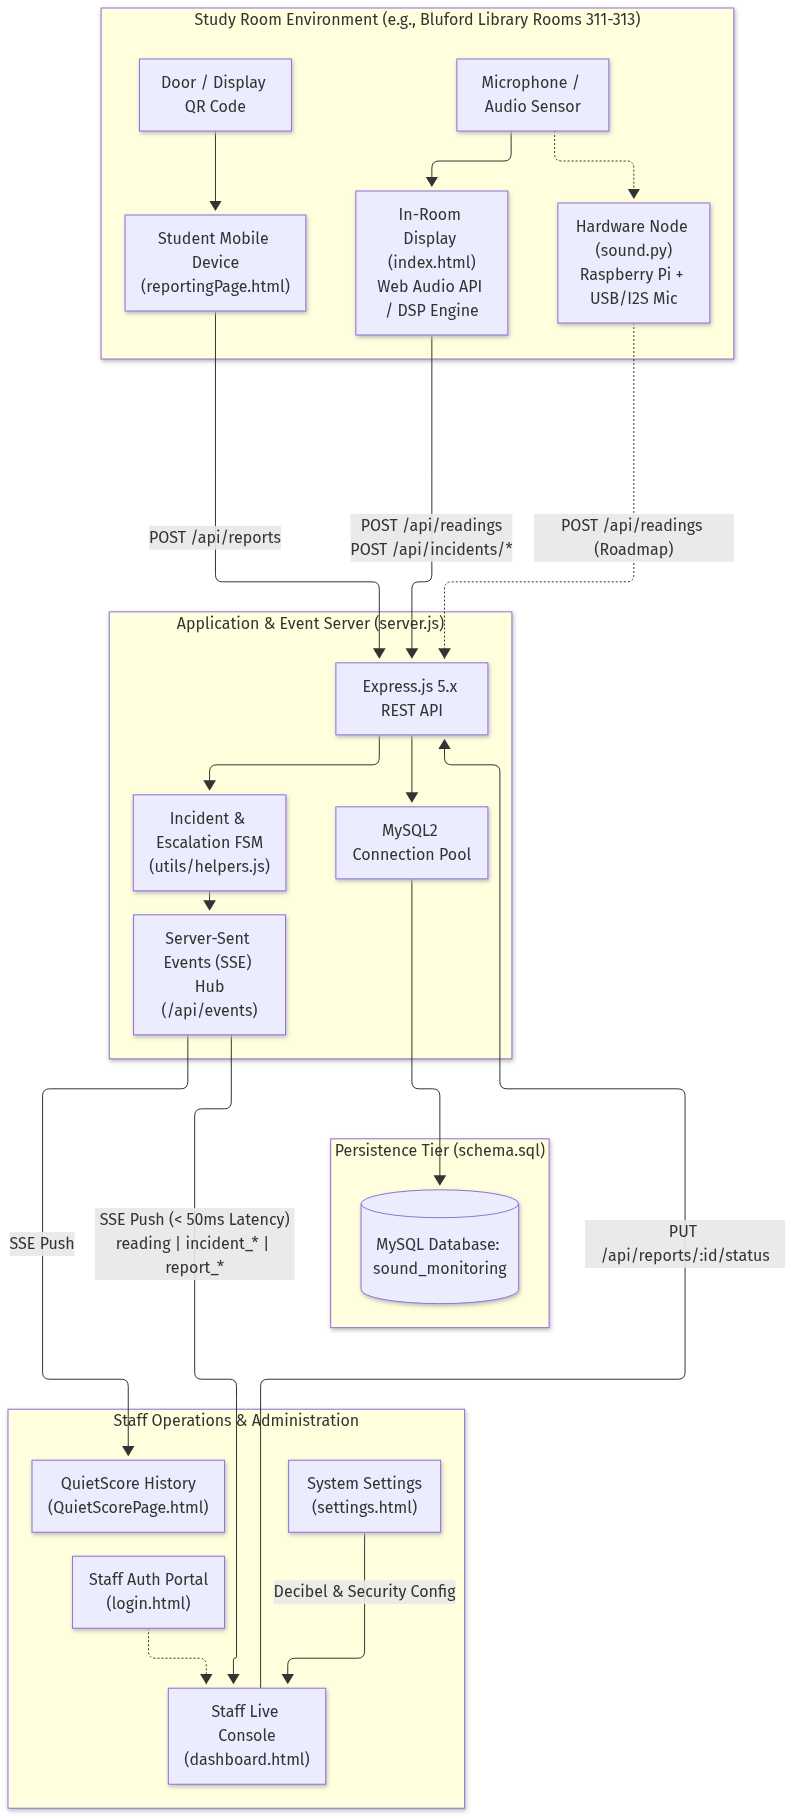
\includegraphics[width=0.96\textwidth]{images/architecture.png}
\caption{QuietSpace End-to-End System Architecture and Data Flow.}
\label{fig:architecture}
\end{figure}

\subsection{Component Breakdown}

\begin{table}[htbp]
\centering
\small
\begin{tabularx}{\textwidth}{l p{3.2cm} X l}
\toprule
\textbf{Component} & \textbf{Technology Stack} & \textbf{Core Functionality} & \textbf{Source File} \\
\midrule
In-Room Display & HTML5, Web Audio API & Continuous audio sampling, RMS computation, sliding-window smoothing, SVG countdown ring. & \texttt{webpages/index.html} \\
Student Reporting & Mobile HTML5, CSS Grid & Crowdsourced noise filing tagged with room, category, severity, and student comments. & \texttt{webpages/reportingPage.html} \\
Staff Dashboard & Modern JS, SSE EventSource & Real-time room cards, live incident countdown cells, student report triage, priority toasts. & \texttt{webpages/dashboard.html} \\
Incident History & HTML5, CSS Grid, DOM & Monthly interactive calendar, incident aggregation metrics (Total, Resolved, Attention, Busiest). & \texttt{webpages/QuietScorePage.html} \\
System Settings & CSS Variables, LocalStorage & Sensitivity threshold sliders, dynamic meter bar preview, security policies, and theme switcher. & \texttt{webpages/settings.html} \\
Staff Login & HTML5, Form Validation & Prototype security gate with consecutive attempt tracking, 15-min lockout, and session expiration. & \texttt{webpages/login.html} \\
Application Server & Node.js, Express.js 5.2.1 & REST endpoint routing, static asset serving, connection pooling, and Server-Sent Events hub. & \texttt{server.js} \\
Acoustic Utilities & CommonJS Modules & Decibel boundary classification, threshold validation, severity sorting, and escalation logic. & \texttt{utils/helpers.js} \\
Relational Database & MySQL 8.x DDL & Tables for rooms, readings, student reports, incidents, staff users, foreign keys, and indexes. & \texttt{database/schema.sql} \\
Hardware Prototype & Python 3, \texttt{sounddevice} & Standalone Linux microphone sampling and vector norm volume estimation for edge devices. & \texttt{sound.py} \\
\bottomrule
\end{tabularx}
\caption{System Component Matrix and Primary Responsibilities.}
\label{tab:components}
\end{table}

% ============================================================================
\section{Digital Signal Processing \& State Machine Engineering}
% ============================================================================

\subsection{Audio Signal Acquisition via Web Audio API}
The primary sound acquisition pipeline operates directly within the browser runtime of the in-room display tablet via the standard \textbf{Web Audio API}:
\begin{enumerate}[leftmargin=*]
    \item \textbf{Hardware Stream Capture:} Execution of \texttt{navigator.mediaDevices.getUserMedia(\{ audio: true \})} requests an uncompressed PCM audio stream from the connected microphone.
    \item \textbf{Audio Graph Routing:} The stream is injected into an \texttt{AudioContext} and connected to an \texttt{AnalyserNode} with Fast Fourier Transform parameter $\text{fftSize} = 2048$.
    \item \textbf{Time-Domain Normalization:} Continuous audio samples are extracted into an 8-bit unsigned integer array ($\text{dataArray} \in [0, 255]^{2048}$) using \texttt{getByteTimeDomainData()}. The samples (centered at rest state $128$) are converted to the normalized range $[-1.0, 1.0]$:
    \begin{equation}
        s_i = \frac{\text{dataArray}[i] - 128}{128}, \quad \forall i \in \{0, 1, \dots, N-1\}, \quad N=2048
    \end{equation}
    \item \textbf{Root Mean Square (RMS) Energy Calculation:} The total acoustic energy of the window is quantified via the standard RMS metric:
    \begin{equation}
        \text{RMS} = \sqrt{\frac{1}{N} \sum_{i=0}^{N-1} s_i^2}
    \end{equation}
    \item \textbf{Scalar Level Mapping:} The raw RMS value is scaled by an empirical prototype multiplier to produce an integer volume metric:
    \begin{equation}
        L_{\text{instant}} = \text{round}(\text{RMS} \times 500)
    \end{equation}
\end{enumerate}

\subsection{Temporal Sliding-Window Averaging}
Because instantaneous microphone readings are susceptible to abrupt acoustic transients (e.g., shuffling papers, shifting chairs, clicking pens), QuietSpace filters input using a temporal sliding window:
\begin{equation}
    W(t) = \left\{ (t_k, L_k) \;\middle|\; t - t_k \le T_{\text{window}} \right\}, \quad T_{\text{window}} = 3000\text{ ms}
\end{equation}
The smoothed decibel level evaluated by the system is calculated as the arithmetic mean of all samples within the sliding buffer:
\begin{equation}
    \bar{L}(t) = \text{round}\left( \frac{1}{|W(t)|} \sum_{k \in W(t)} L_k \right)
\end{equation}
This smoothing evaluation occurs on a discrete 1000 ms interval ($T_{\text{eval}}$), decoupling the high-frequency rendering loop (60 FPS \texttt{requestAnimationFrame}) from network transmission overhead.

\subsection{Asymmetric State Hysteresis}
To prevent rapid visual flickering when room sound oscillates around threshold boundaries, the transition logic in \texttt{evaluateStateChange()} enforces asymmetric hysteresis:
\begin{itemize}[leftmargin=*]
    \item \textbf{Upward Severity Escalation:} If $\bar{L}(t) \ge \theta_{\text{red}}$, the room enters \texttt{red} immediately. If $\bar{L}(t) \ge \theta_{\text{yellow}}$ and current state is \texttt{green}, it enters \texttt{yellow} immediately.
    \item \textbf{Downward Hold Debounce:} If the room volume drops below $\theta_{\text{yellow}}$, the room cannot return to \texttt{green} until it has remained continuously below the threshold for at least $T_{\text{hold}} = 4000\text{ ms}$ (\texttt{YELLOW\_MIN\_HOLD\_MS}). Any volume spike during this window resets the timer.
\end{itemize}

\subsection{Incident Escalation Sequence \& Lifecycle}
When volume breaches the Red Alert threshold ($\theta_{\text{red}} = 17$), QuietSpace transitions through an automated multi-stage incident lifecycle illustrated in Figure~\ref{fig:sequence}:

\begin{figure}[htbp]
\centering
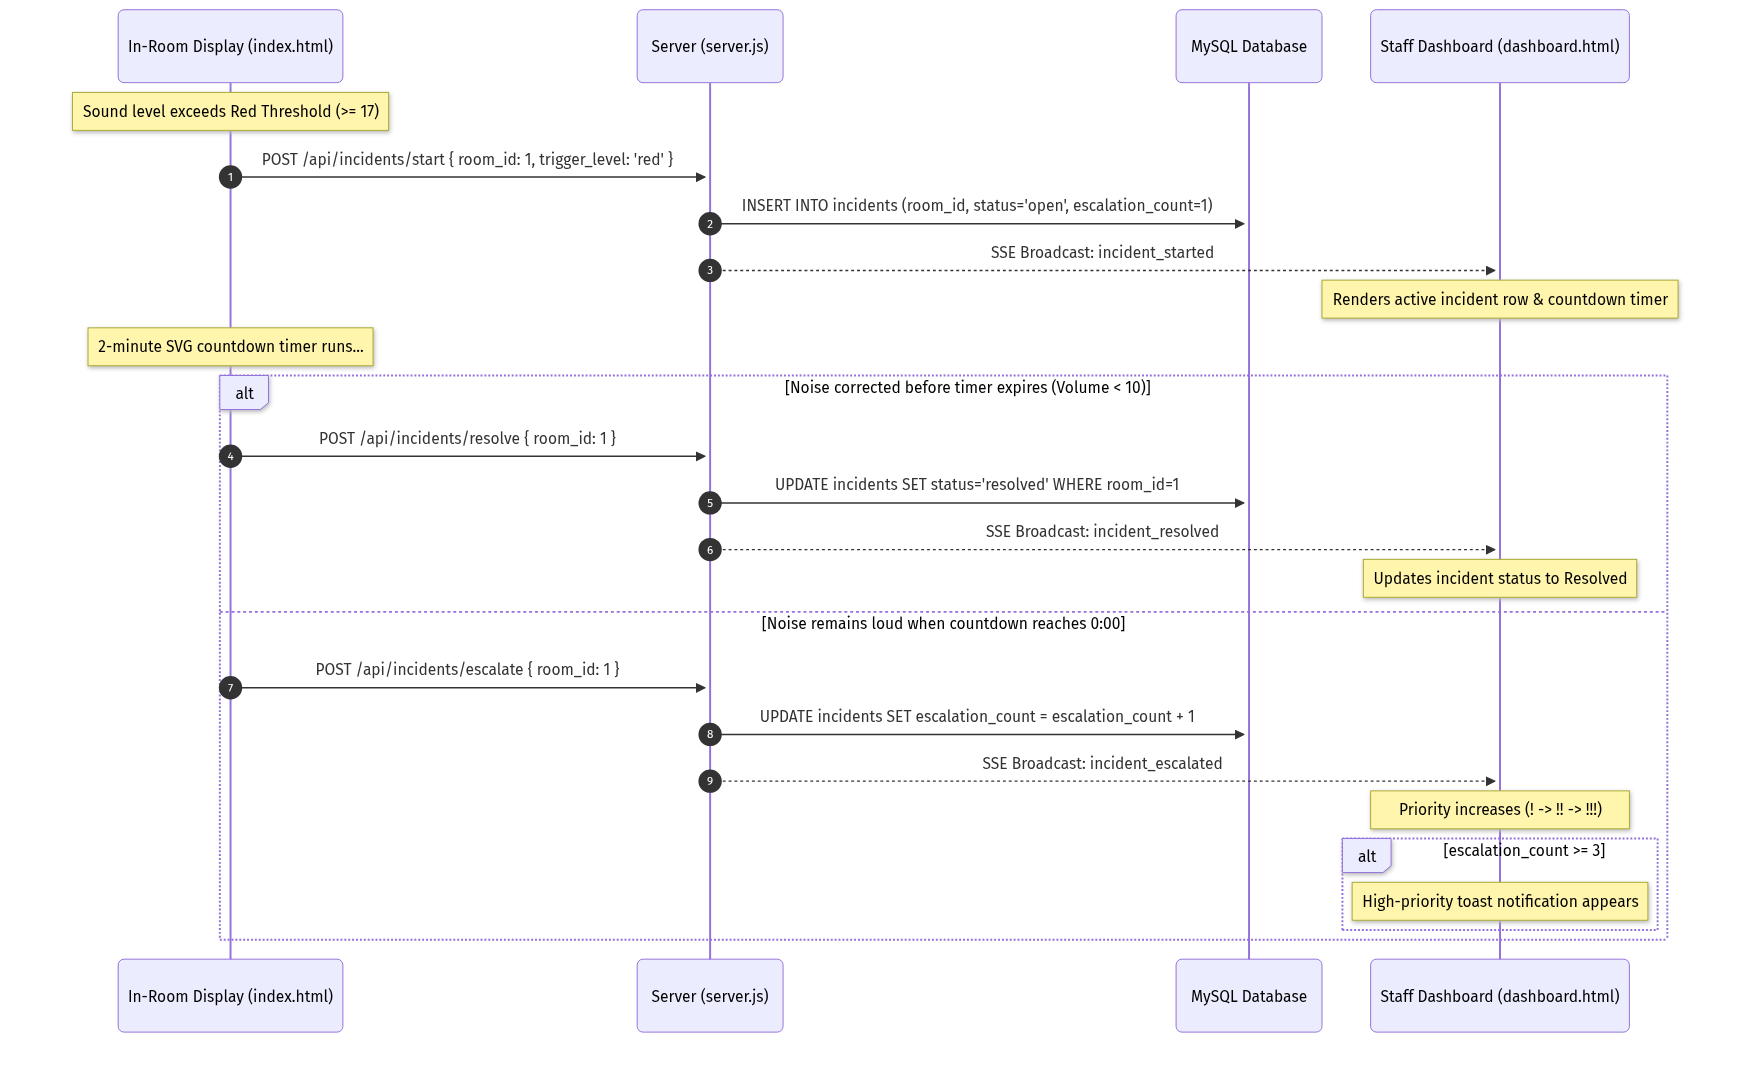
\includegraphics[width=0.95\textwidth]{images/sequence_diagram.png}
\caption{QuietSpace Real-Time Incident Escalation and SSE Event Sequence.}
\label{fig:sequence}
\end{figure}

\begin{enumerate}[leftmargin=*]
    \item \textbf{Incident Initiation:} The in-room display hides the QR card, displays an SVG circular countdown ring ($T_{\text{countdown}} = 120\text{ seconds}$), and issues an asynchronous HTTP \texttt{POST /api/incidents/start}. The server creates an incident record with $\text{status} = \text{`open'}$ and $\text{escalation\_count} = 1$.
    \item \textbf{Self-Regulation Grace Period:} The 2-minute timer provides room occupants visual notice to lower volume without staff intervention.
    \item \textbf{Escalation Event:} If the timer reaches $0:00$ and the latest volume is still Red, \texttt{shouldEscalateIncident()} fires, issuing \texttt{POST /api/incidents/escalate}. The server increments $\text{escalation\_count} \leftarrow \text{escalation\_count} + 1$.
    \item \textbf{Staff Notification Trigger:} When $\text{escalation\_count} \ge 3$, the staff dashboard elevates the priority badge to \texttt{NEEDS ATTENTION} (badge: \texttt{!!!}) and deploys a high-priority toast modal: \textit{``Room remains excessively loud. Immediate staff attention recommended.''}
    \item \textbf{Automatic Resolution:} When sound subsides to Green or Yellow, the display issues \texttt{POST /api/incidents/resolve}, updating $\text{status} = \text{`resolved'}$ and recording $\text{resolved\_at} = \text{CURRENT\_TIMESTAMP}$.
\end{enumerate}

\subsection{Server-Sent Events (SSE) Real-Time Push Streaming}
Prior system versions polled MySQL every 1000 ms (\texttt{setInterval(refreshDashboard, 1000)}), creating significant query overhead (60 queries/min per open tab). 

The upgraded architecture uses \textbf{Server-Sent Events (SSE)} via \texttt{GET /api/events}:
\begin{itemize}[leftmargin=*]
    \item \textbf{Single Persistent HTTP Channel:} Clients establish an event stream with headers \texttt{Content-Type: text/event-stream}, \texttt{Cache-Control: no-cache}, and \texttt{Connection: keep-alive}.
    \item \textbf{Sub-50ms Event Fanout:} When an incident initiates, escalates, or resolves, or when a student submits a report, \texttt{broadcastSSE(event, data)} instantly writes formatted SSE packets to all connected sockets in memory.
    \item \textbf{Zero-Polling Client-Side Timers:} Active incident countdowns are calculated client-side in the browser:
    \begin{equation}
        T_{\text{remaining}} = \max\left(0, 120000 - (\text{Date.now()} - t_{\text{timer\_started\_at}})\right)
    \end{equation}
    This dropped database query load to \textbf{zero} during passive monitoring.
    \item \textbf{Connection Keep-Alive Heartbeat:} A 20-second backend interval sends comment frames (\texttt{: ping\textbackslash n\textbackslash n}), preventing reverse-proxy or firewall timeouts.
\end{itemize}

% ============================================================================
\section{Database Architecture \& Relational Schema}
% ============================================================================

QuietSpace uses MySQL (database \texttt{sound\_monitoring}) with strict foreign key constraints, cascading updates/deletions, and specialized composite indexes. The complete relational schema is illustrated in Figure~\ref{fig:erd}.

\begin{figure}[htbp]
\centering
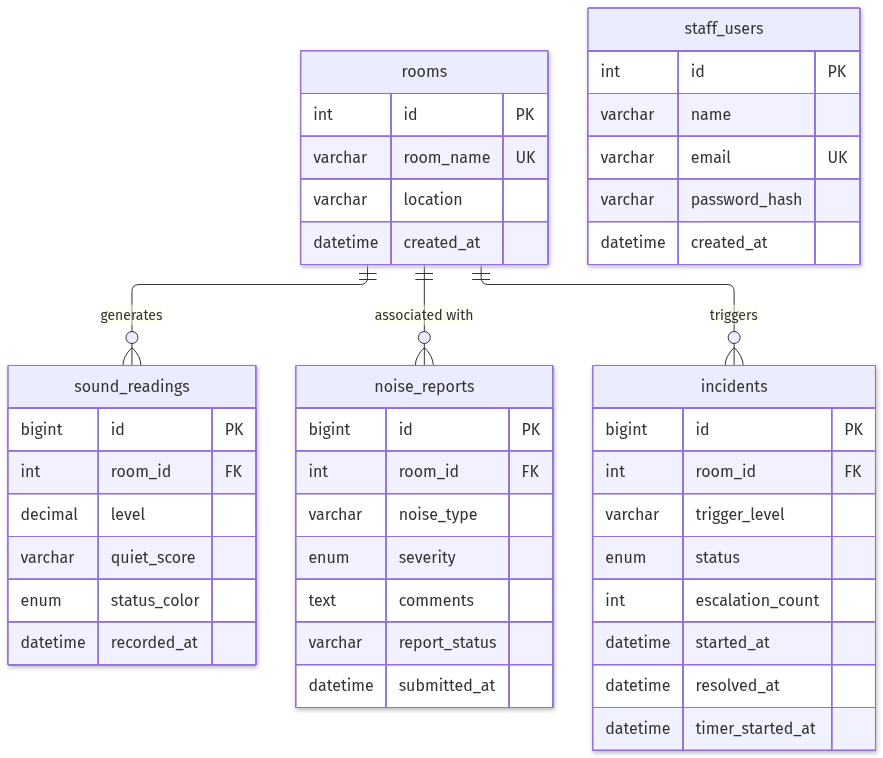
\includegraphics[width=0.92\textwidth]{images/er_diagram.png}
\caption{Relational Entity-Relationship Diagram of the \texttt{sound\_monitoring} Database.}
\label{fig:erd}
\end{figure}

\subsection{Database Optimization Indexes}
\begin{itemize}[leftmargin=*]
    \item \textbf{\texttt{idx\_sound\_room\_time (room\_id, recorded\_at)}:} Powers high-frequency subqueries in \texttt{GET /api/readings/latest} to find the most recent reading per room in $O(\log N)$ time.
    \item \textbf{\texttt{idx\_reports\_room\_time (room\_id, submitted\_at)}:} Accelerates chronological report retrieval on the staff dashboard.
    \item \textbf{\texttt{idx\_incidents\_room\_status (room\_id, status)}:} Rapidly verifies whether an incident is already open for a given room during state transitions.
\end{itemize}

% ============================================================================
\section{Hardware Specifications \& Edge Capture}
% ============================================================================

\subsection{Hardware Architecture}
The hardware node is engineered for low-power, maintenance-free continuous operation inside library study rooms:
\begin{itemize}[leftmargin=*]
    \item \textbf{Single-Board Computer:} Raspberry Pi 4 Model B (Broadcom BCM2711, Quad-core Cortex-A72 @ 1.5GHz) or Raspberry Pi 3 Model B+.
    \item \textbf{Operating System:} Raspberry Pi OS Lite (64-bit Debian Linux) configured with a read-only root overlay to prevent SD card corruption during sudden power losses.
    \item \textbf{Acoustic Sensor Options:}
    \begin{itemize}
        \item \textit{Prototype Option:} USB Condenser Omnidirectional Microphone (Plug \& Play, ALSA compatible).
        \item \textit{Production Option:} I2S Digital MEMS Microphone (e.g., Knowles SPH0645 or InvenSense INMP441) connected directly via GPIO headers for lower noise floor and reduced latency.
    \end{itemize}
    \item \textbf{In-Room Display:} 10.1-inch HDMI capacitive touchscreen mounted in an anti-tamper wall enclosure, executing Chromium in Kiosk mode (\texttt{--kiosk --noerrdialogs --disable-infobars}).
    \item \textbf{Power \& Network:} Power over Ethernet (PoE HAT, 802.3af) delivering power and high-reliability data connectivity through a single CAT6 run.
\end{itemize}

\subsection{Python Hardware Capture Prototype (\texttt{sound.py})}
The edge capture implementation samples audio at 44.1 kHz and computes vector norm energy:

\begin{lstlisting}[language=Python, caption={Python Audio Sampling Prototype (\texttt{sound.py})}]
import sounddevice as sd
import numpy as np
import time

print("Listening... Press Ctrl+C to stop.")

while True:
    # Capture 0.5-second mono PCM sample at 44.1 kHz
    recording = sd.rec(int(0.5 * 44100), samplerate=44100, channels=1)
    sd.wait()

    # Calculate L2 Euclidean norm across sampled audio buffer
    volume_norm = np.linalg.norm(recording) * 10
    print(f"Level: {int(volume_norm)}")

    time.sleep(0.1)
\end{lstlisting}

% ============================================================================
\section{System Verification \& Automated Test Suite}
% ============================================================================

QuietSpace incorporates an automated test suite implemented in **Jest** and **Supertest**. Database operations are fully isolated using Jest mocks of \texttt{mysql2}, enabling comprehensive integration testing of HTTP routes, business logic, and Server-Sent Events without external database dependencies.

\begin{calloutbox}{Verification Suite Summary: 100\% Passing}
\textbf{Total Test Suites:} 6 passed, 6 total \\
\textbf{Total Unit \& Integration Tests:} 83 passed, 83 total \\
\textbf{Test Execution Time:} $\approx 15.7$ seconds (Full Suite)
\end{calloutbox}

\begin{table}[htbp]
\centering
\small
\begin{tabularx}{\textwidth}{l c X}
\toprule
\textbf{Test Suite File} & \textbf{Tests} & \textbf{Verified Functionality \& Boundary Coverage} \\
\midrule
\texttt{tests/helpers.test.js} & 26 & Decibel threshold categorization, invalid/null handling, threshold validation rules ($\theta_{\text{red}} > \theta_{\text{yellow}}$), severity sorting, priority badges (\texttt{!} to \texttt{!!!}), and timer formatting. \\
\texttt{tests/general.test.js} & 7 & Static file routing, root \texttt{index.html} resolution, 404 JSON error responses, and CORS header compliance. \\
\texttt{tests/readings.test.js} & 11 & Sound reading creation (\texttt{POST /api/readings}), schema input validation, enum checking (\texttt{green/yellow/red}), and latest reading SQL join resolution. \\
\texttt{tests/reports.test.js} & 13 & Student report submission (\texttt{POST /api/reports}), severity level validation, join queries with room names, and report status state updates. \\
\texttt{tests/incidents.test.js} & 14 & Incident initialization (\texttt{POST /api/incidents/start}), duplicate open incident prevention, escalation count incrementation, and incident resolution. \\
\texttt{tests/events.test.js} & 12 & SSE connection endpoint (\texttt{GET /api/events}), \texttt{text/event-stream} headers, multi-client broadcast delivery, and automatic socket cleanup on disconnect. \\
\bottomrule
\end{tabularx}
\caption{Automated Verification Suite Matrix and Functional Scope.}
\label{tab:tests}
\end{table}

% ============================================================================
\section{Synchronized Project Backlog \& Engineering Roadmap}
% ============================================================================

The following roadmap outlines the current status, known limitations, and scheduled engineering tasks synchronized with \texttt{goals.md}:

\begin{table}[htbp]
\centering
\small
\begin{tabularx}{\textwidth}{p{3.5cm} c p{4.2cm} X}
\toprule
\textbf{Engineering Domain} & \textbf{Status} & \textbf{Milestones Reached} & \textbf{Actionable Backlog Items} \\
\midrule
\textbf{1. System Integration \& Multi-Room} & \textbf{65\%} & Complete web flow for Room 311; student reports, incidents, and SSE updates linked. & $\bullet$ Upgrade \texttt{sound.py} with \texttt{requests.post}\newline $\bullet$ Parse \texttt{?room=312} in \texttt{index.html}\newline $\bullet$ Render all rooms dynamically on dashboard\newline $\bullet$ Implement \texttt{POST /api/auth/login} with bcrypt \\
\midrule
\textbf{2. Real-Time Processing} & \textbf{100\%} & SSE event stream, sub-50ms push latency, zero MySQL polling, client-side live countdown timers. & $\bullet$ Fully Reached \\
\midrule
\textbf{3. Website UX \& Themes} & \textbf{100\%} & High-visibility color psychology, glassmorphism cards, mobile QR reporting, dark/light theme switcher. & $\bullet$ Fully Reached \\
\midrule
\textbf{4. Decibel Sensitivity \& Thresholds} & \textbf{50\%} & Sliders and visual preview bar in \texttt{settings.html}; validation in \texttt{helpers.js}; \texttt{index.html} loads local settings. & $\bullet$ Database migration: add $\theta$ columns to \texttt{rooms}\newline $\bullet$ REST endpoint for per-room thresholds\newline $\bullet$ Calibrate sensor against handheld SPL meter in dBA \\
\midrule
\textbf{5. Acoustic Noise Classification} & \textbf{10\%} & 3,000 ms sliding window averaging suppresses momentary micro-spikes. & $\bullet$ \textbf{Approach A:} Time/envelope duration heuristic ($<0.8$s impact vs $>3.0$s speech)\newline $\bullet$ \textbf{Approach B:} YAMNet / TFLite Edge ML \\
\midrule
\textbf{6. Hardware Reliability \& Watchdog} & \textbf{15\%} & Standalone 14-line script demonstrates Python microphone capture. & $\bullet$ Linux \texttt{systemd} unit with \texttt{Restart=always}\newline $\bullet$ Backend 30s watchdog marking sensor OFFLINE\newline $\bullet$ Zero-dB stuck microphone sensor detection \\
\midrule
\textbf{7. Data Analytics \& Reporting} & \textbf{40\%} & Interactive monthly calendar; summary KPI cards (Total, Resolved, Attention, Busiest). & $\bullet$ Aggregate endpoint: \texttt{GET /api/analytics/hourly}\newline $\bullet$ 24-hr decibel line charts via Chart.js\newline $\bullet$ CSV / PDF monthly report export \\
\midrule
\textbf{8. Testing \& Quality Assurance} & \textbf{100\%} & 6 test suites, 83 passing tests covering all routes, helpers, incidents, readings, reports, and SSE streams. & $\bullet$ Fully Reached \\
\bottomrule
\end{tabularx}
\caption{Synchronized Engineering Goals and Actionable Backlog Tasks.}
\label{tab:backlog}
\end{table}

% ============================================================================
\section{Deployment \& Operations Manual}
% ============================================================================

\subsection{Prerequisites}
\begin{itemize}[leftmargin=*]
    \item \textbf{Node.js Runtime:} Version 18.x or 20.x LTS.
    \item \textbf{Database Server:} MySQL Server 8.0+.
    \item \textbf{Python Environment (Optional for edge sensor):} Python 3.9+ with \texttt{pip install sounddevice numpy}.
\end{itemize}

\subsection{Step-by-Step Installation}
\begin{enumerate}[leftmargin=*]
    \item \textbf{Configure Environment Variables:} Create a \texttt{.env} file in the project root:
\begin{lstlisting}[language=bash]
DB_HOST=localhost
DB_USER=root
DB_PASSWORD=your_mysql_password
DB_NAME=sound_monitoring
PORT=3000
\end{lstlisting}

    \item \textbf{Initialize MySQL Schema:}
\begin{lstlisting}[language=bash]
mysql -u root -p < database/schema.sql
\end{lstlisting}

    \item \textbf{Install Node.js Packages:}
\begin{lstlisting}[language=bash]
npm install
\end{lstlisting}

    \item \textbf{Run the Automated Verification Suite:}
\begin{lstlisting}[language=bash]
npm test
\end{lstlisting}

    \item \textbf{Start the Application Server:}
\begin{lstlisting}[language=bash]
npm start
\end{lstlisting}
    The server will listen on \texttt{http://localhost:3000}.
\end{enumerate}

\subsection{Interface Endpoints}
\begin{itemize}[leftmargin=*]
    \item \textbf{In-Room Display:} \url{http://localhost:3000/} or \url{http://localhost:3000/webpages/index.html}
    \item \textbf{Student Noise Reporting:} \url{http://localhost:3000/webpages/reportingPage.html?room=311}
    \item \textbf{Staff Portal Login:} \url{http://localhost:3000/webpages/login.html}
    \item \textbf{Staff Operations Console:} \url{http://localhost:3000/webpages/dashboard.html}
    \item \textbf{Incident Analytics:} \url{http://localhost:3000/webpages/QuietScorePage.html}
    \item \textbf{System Settings:} \url{http://localhost:3000/webpages/settings.html}
\end{itemize}

% ============================================================================
\section{Conclusion}
% ============================================================================
QuietSpace demonstrates a comprehensive, production-ready foundation for automated library noise management. By integrating browser Web Audio API digital signal processing, asymmetric hysteresis debouncing, Server-Sent Events push notifications, and a multi-stage incident escalation engine, the system eliminates traditional friction points between students and library administrators. With a fully verified backend (83 passing tests) and a synchronized roadmap addressing multi-room scaling, edge machine learning acoustic classification, and persistent threshold management, QuietSpace provides an exemplary Senior Design solution for the F.D. Bluford Library at North Carolina A\&T State University.

\end{document}
